 \documentclass[12pt]{article}
\usepackage{amsmath}
\usepackage{amssymb}
\usepackage{geometry}
\usepackage{amsmath, amsfonts, bm, graphicx}
\usepackage{tabularx}
\usepackage{booktabs} 
\usepackage{float}
\usepackage{enumitem,cancel}
\geometry{margin=1in}


\title{}
\date{}
\author{}
\DeclareMathOperator{\Real}{Re}
\DeclareMathOperator{\Imag}{Im}

\begin{document}
\subsection*{\boxed{\text{HW 9 - Zeshui Song}}}
\underline{Notes:}
\begin{itemize}
    \item \textbf{Dot Convention for Mutual Inductance}:
    \begin{itemize}
        \item A current entering the \textit{dotted} terminal of one coil produces an open-circuit voltage with a positive voltage reference at the \textit{dotted} terminal of the second coil.
        \item A current entering the \textit{undotted} terminal of one coil provides a voltage that is positively sensed at the \textit{undotted} terminal of the second coil
    \end{itemize}
    \begin{center}
        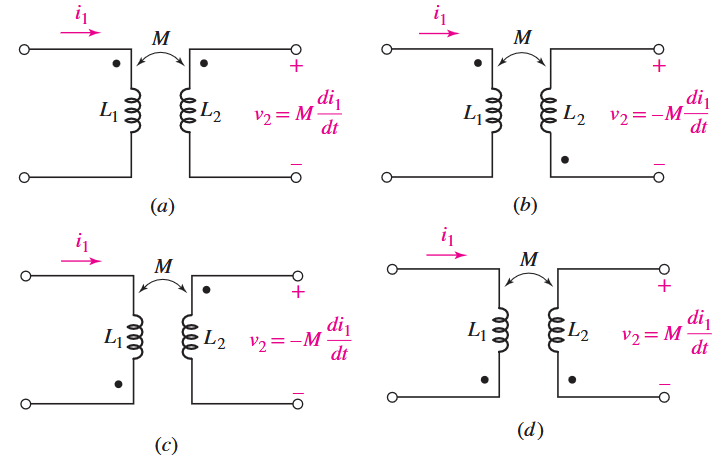
\includegraphics[width=0.8\textwidth]{dot.png}
    \end{center}
    Note that \textbf{self-induction} exists if the current in the right loop ($i_2$) is non-zero and would cause back emf.
    \item Combining mutual and self-induction:
    \begin{center}
        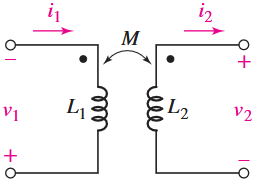
\includegraphics[width=0.4\textwidth]{combine.png}
    \end{center}
    By passive current convention, current $i_1$ should enter the positive terminal of the inductor $L_1$. However, the polarity of $v_1$ indicates that $di_1/dt$ must be negative (indicating current flowing in the opposite direction). By the dot convention, current $i_2$ enters the undotted terminal of $L_2$, so the mutual inductance contribution to $v_1$ is positive by the polarity of $v_1$. 
    \[v_1 = -L_1\frac{di_1}{dt} + M\frac{di_2}{dt}\]
    Similarly for $v_2$:
    \[v_2 = -L_2\frac{di_2}{dt} + M\frac{di_1}{dt}\]
    These same sign conventions apply to sinusoidal steady-state analysis, where $i_1$ and $i_2$ are phasors.
    \[\mathbf{V_1} = -j\omega L_1 \mathbf{I_1} + j\omega M \mathbf{I_2}\]
    \[\mathbf{V_2} = -j\omega L_2 \mathbf{I_2} + j\omega M \mathbf{I_1}\]
    \item Total energy in coupled inductors:
    \begin{center}
        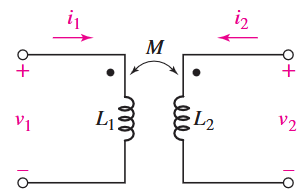
\includegraphics[width=0.4\textwidth]{energy.png}
    \end{center}
    \[w(t)=\frac{1}{2}L_1[i_1(t)]^2 + \frac{1}{2}L_2[i_2(t)]^2 + M[i_1(t)][i_2(t)]\]
    \textbf{Limit on M}:
    \[M \leq \sqrt{L_1 L_2}\]
    \textbf{Coupling coefficient:}
    \[k = \frac{M}{\sqrt{L_1 L_2}} \implies 0 \leq k \leq 1\]
    \item Linear transformer and reflected impedance:
    \begin{center}
        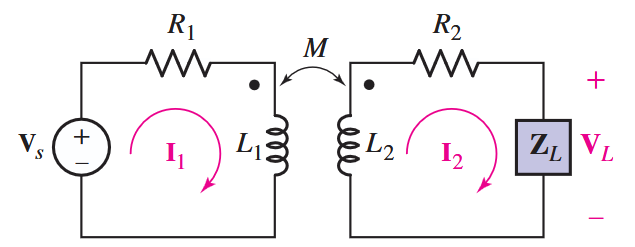
\includegraphics[width=0.6\textwidth]{transformer.png}
    \end{center}
    The \textit{primary circuit} contains the source $v_s$ and the \textit{secondary circuit} contains the load $\mathbf{V_L}$.\\\\
    By using mesh analysis on each of the two loops, we can simplify the circuit to an equivalent circuit with a $\mathbf{V_s}$ in series with a reflected impedance $\mathbf{Z_\text{in}}$:
    \[\frac{\mathbf{V_s}}{\mathbf{I_1}} = \mathbf{Z_\text{in}} = \mathbf{Z_{11}}-\frac{(j\omega)^2M^2}{\mathbf{Z_{22}}}\]
    Where $\mathbf{Z_{11}}$ and $\mathbf{Z_{22}}$ are the self-impedances of the primary and secondary circuits, respectively. 
    \[\mathbf{Z_{11}} = R_1+j\omega L_1\]
    \[\mathbf{Z_{22}} = R_2+j\omega L_2 + \mathbf{Z_L}\]
    \item \textbf{Ideal Transformer}:
    \begin{center}
        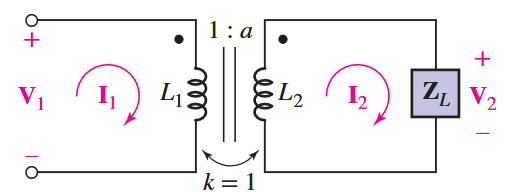
\includegraphics[width=0.6\textwidth]{ideal.png}
    \end{center}
    In an ideal transformer, the coupling coefficient $k=1$ and the mutual inductance $M = \sqrt{L_1 L_2}$.\\\\
    \textbf{Turns Ratio:}
    \[a^2 = \frac{L_2}{L_1} = \frac{N_2^2}{N_1^2}\]
    Using turns ratio, we can have the following relationships:
    \[\frac{1}{a} = \frac{I_2}{I_1}\]
    \[a = \frac{V_2}{V_1}\]
    \[a^2 = \frac{\mathbf{Z_L}}{\mathbf{Z_\text{in}}}\]
\end{itemize}

\section*{13.6}
\vspace{-2em}
\begin{center}
    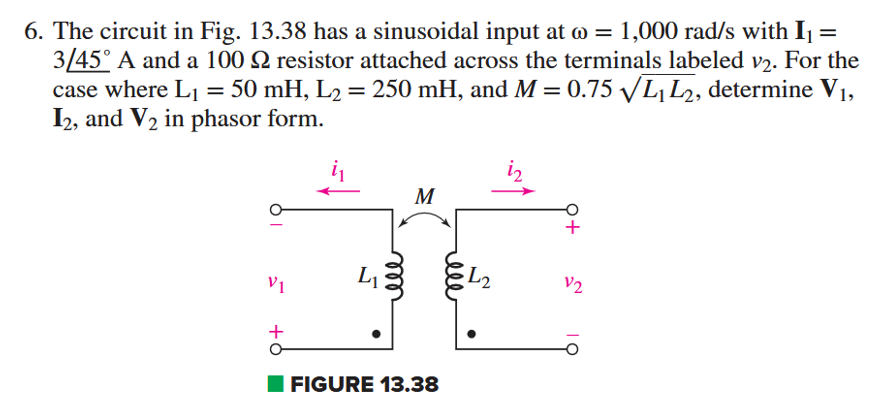
\includegraphics[width=0.8\textwidth]{13-6.png}
\end{center}
This is a circuit at sinusoidal steady state, so we can use phasor analysis. First, defining constants and impedances:
\begin{itemize}
    \item $\omega = 1000$ rad/s
    \item $\mathbf{I_1} = 3\angle 45^\circ $ A 
    \item Resistor across $v_2$: $R=100 \Omega$
    \item $L_1 = 50$ mH $\implies \mathbf{Z_{L1}} = j\omega L_1 = 50j$ $\Omega$
    \item $L_2 = 250$ mH $\implies \mathbf{Z_{L2}} = j\omega L_2 = 250j$ $\Omega$
    \item $M = 0.75\sqrt{L_1L_2} = 83.852$ mH $\implies \mathbf{Z_M} = j\omega M = 83.852j$ $\Omega$
\end{itemize}
Instead of following the current direction defined in the diagram, I will redraw the circuit following passive sign convention. At the end, I will map my results back to the original diagram with a sign change if necessary.
\begin{center}
    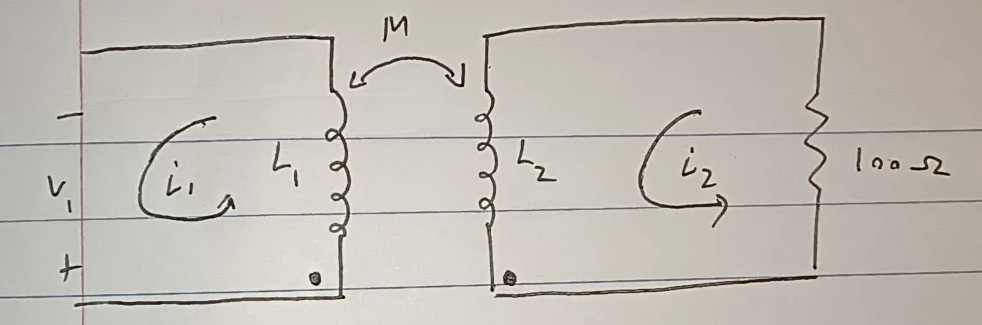
\includegraphics[width=0.6\textwidth]{13-6-1.png}
\end{center}
\textbf{KVL to mesh 1:}
\[\mathbf{V_1} - \mathbf{Z_{L1}}\mathbf{I_1} + \mathbf{Z_M}\mathbf{I_2} = 0\]
\[\mathbf{V_1} - [50j \,\Omega]\mathbf{I_1} + [83.852j \,\Omega]\mathbf{I_2} = 0\]
\[\mathbf{V_1}  + [83.852j \,\Omega]\mathbf{I_2} = [50j \,\Omega]\mathbf{I_1}\]
Converting to polar form for easier multiplication:
\[[50j \,\Omega]\mathbf{I_1} = (50\angle 90^\circ)(3\angle 45^\circ) = 150\angle 135^\circ = -106.07 + 106.07j\]
\[\implies \mathbf{V_1} + (83.852j)\mathbf{I_2} = (-106.07 + 106.07j)\]
\textbf{KVL to mesh 2:}
\[-\mathbf{I_2}R - \mathbf{Z_{L2}}\mathbf{I_2} + \mathbf{Z_M}\mathbf{I_1} = 0\]
\[-\mathbf{I_2}[100 \,\Omega] - [250j \,\Omega]\mathbf{I_2} + [83.852j \,\Omega]\mathbf{I_1} = 0\]
\[0\mathbf{V_1}+ (-100-250j)\mathbf{I_2}=-(83.852j)\mathbf{I_1}\]
Converting to polar form for easier multiplication:
\[-(83.852j)\mathbf{I_1}= -(83.852\angle 90^\circ)(3\angle 45^\circ) = -251.556\angle 135^\circ = 177.87 - 177.87j\]
\[\implies 0\mathbf{V_1} + (-100-250j)\mathbf{I_2} = (177.87 - 177.87j)\]
Solving this system of equations, we get:
\[\mathbf{V_1} = -34.067 + 75.211j \text{ V} \implies 82.56\angle 114.36^\circ\]
\[\mathbf{I_2} = 0.368 + 0.858j \text{ A} \implies 0.933\angle 66.78^\circ\]
\[\implies \mathbf{V_2} = \mathbf{I_2}R = 93.3\angle 66.78^\circ \text{ V}\]
Mapping back to the original diagram, we have:
\[\boxed{\mathbf{V_1} = 82.56\angle 114.36^\circ}\]
\[\boxed{\mathbf{I_2} = -0.933\angle 66.78^\circ}\]
\[\boxed{\mathbf{V_2} = -93.3\angle 66.78^\circ \text{ V}}\]

\newpage
\section*{13.17}
\vspace{-2em}
\begin{center}
    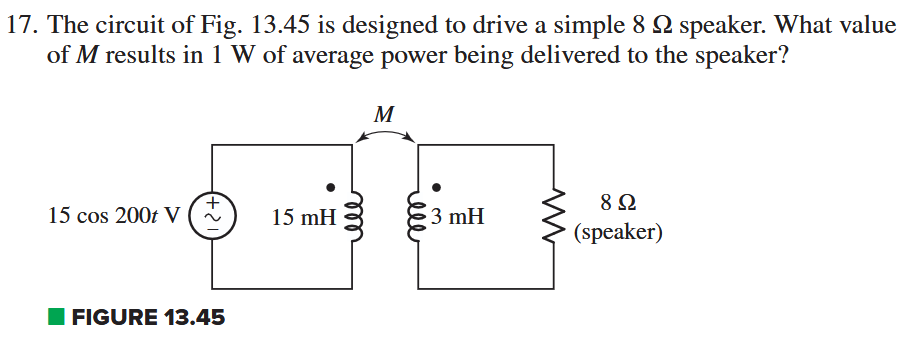
\includegraphics[width=0.8\textwidth]{13-17.png}
\end{center}
Defining impedances and constants:
\begin{itemize}
    \item $\mathbf{V_s} = 15\angle 0^\circ$ V
    \item $\omega = 200$ rad/s
    \item $L_1 = 15$ mH $\implies \mathbf{Z_{L1}} = j\omega L_1 = 3j$ $\Omega$
    \item $L_2 = 3$ mH $\implies \mathbf{Z_{L2}} = j\omega L_2 = 0.6j$ $\Omega$
    \item $M\leq \sqrt{L_1 L_2}= 6.7\text{ mH} $ $\implies \mathbf{Z_M} = j\omega M=200Mj $ $\Omega$
\end{itemize}
\begin{center}
    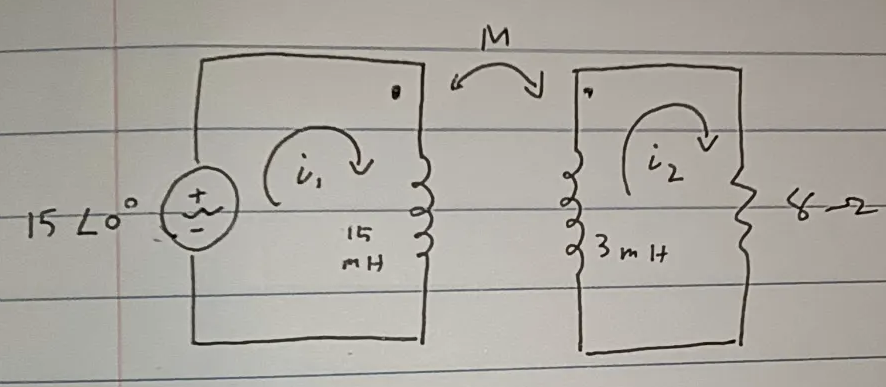
\includegraphics[width=0.6\textwidth]{13-17-1.png}
\end{center}
The average power delivered to the speaker is given by:
\[P_\text{avg} = I_\text{rms}^2 R = \frac{I_\text{max}^2 R}{2}, \quad I_\text{rms} = \frac{I_\text{max}}{\sqrt{2}}\]
\[\implies P_\text{avg} = \frac{1}{2}|\mathbf{I_2}|^2R\]
\[\implies |\mathbf{I_2}|^2 = \frac{2P_\text{avg}}{R} = \frac{2[1\,\text{W}]}{[8\,\Omega]}\implies |\mathbf{I_2}| = 0.5\]
Thus, using mesh analysis we can solve for $\mathbf{I_2}$ and then calculate $P_\text{avg}$ in terms of $M$:\\
\textbf{KVL to mesh 1:}
\[\mathbf{V_s} - \mathbf{Z_{L1}}\mathbf{I_1} + \mathbf{Z_M}\mathbf{I_2} = 0\]
\[(15) - (3j)\mathbf{I_1} + (200Mj)\mathbf{I_2} = 0\]
\[\mathbf{I_1} = \frac{15}{3j}+\frac{200Mj}{3j}\mathbf{I_2} = -5j+66.66M\mathbf{I_2}\]
\textbf{KVL to mesh 2:}
\[-\mathbf{I_2}R - \mathbf{Z_{L2}}\mathbf{I_2} + \mathbf{Z_M}\mathbf{I_1} = 0\]
\[-(8)\mathbf{I_2} - (0.6j)\mathbf{I_2} + (200Mj)\mathbf{I_1} = 0\]
Plug in $\mathbf{I_1}$ from the first equation:
\[(-8-0.6j)\mathbf{I_2} + (200Mj)(-5j+66.66M\mathbf{I_2}) = 0\]
\[(-8-0.6j)\mathbf{I_2} + 1000M+13333M^2j\mathbf{I_2} = 0\]
\[\mathbf{I_2} = \frac{-1000M}{-8-0.6j+13333M^2j}\]
Now find magnitude of $\mathbf{I_2}$:
\[|\mathbf{I_2}| = \frac{|-1000M|}{|-8-0.6j+13333M^2j|} = \frac{1000M}{\sqrt{(-8)^2 + (-0.6+13333M^2)^2}} = 0.5\]
Solve for $M$:
\[\frac{10^6M^2}{(-8)^2 + (-0.6+13333M^2)^2} = 0.25\]
\[10^6M^2 = 0.25[(-8)^2 + (-0.6+13333M^2)^2]\]
\[10^6M^2 = 0.25[64 + 0.36-1.59\times10^4M^2+1.77\times10^9M^4]\]
\[\implies 4.442\times10^8 M^4 -1.00\times10^6M^2 + 16 = 0\]
Using the quadratic formula to solve for $x = M^2$:
\[\implies 4.442\times10^8 x^2 -1.00\times10^6x + 16 = 0\]
\[x = \frac{10^6\pm \sqrt{10^{12} - 4(4.442\times10^8)(16)}}{2(4.442\times10^8)}\]
\[\implies M^2 = x = 2.235\times10^{-3}, 0.016\times10^{-3}\]
Since $M^2$ cannot be greater than $L_1L_2 =0.045\times10^{-3}$, we have:
\[M^2 = 0.016\times10^{-3} \implies \boxed{M = 4.014\text{ mH}}\]
\newpage

\section*{13.41}
\vspace{-2em}
\begin{center}
    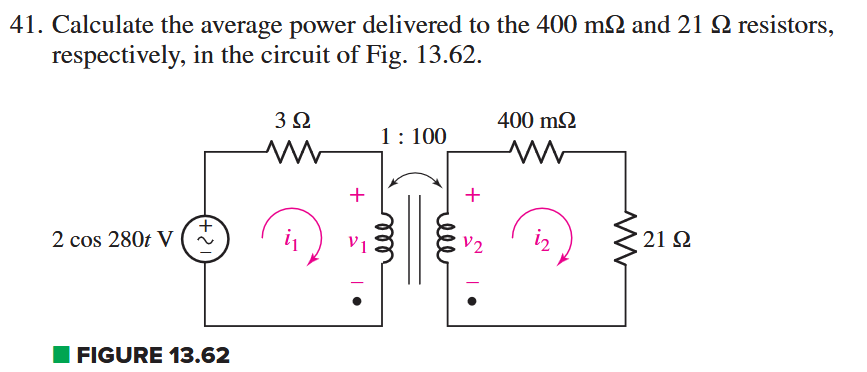
\includegraphics[width=0.8\textwidth]{13-41.png}
\end{center}
Here, we can use the turns ratio $a$ to find the reflected impedance $\mathbf{Z_\text{in}}$:
\[a^2 = \frac{\mathbf{Z_L}}{\mathbf{Z_\text{in}}}\]
Where $a = 100$ and
\[\mathbf{Z_L} = [0.4\,\Omega] + [21\,\Omega] = [21.4\,\Omega]\]
Thus, 
\[\mathbf{Z_\text{in}} = \frac{\mathbf{Z_L}}{a^2} = \frac{21.4}{100^2} = 0.00214\,\Omega\]
We can now redraw the circuit with the reflected impedance to find the current $\mathbf{I_1}$:
\begin{center}
    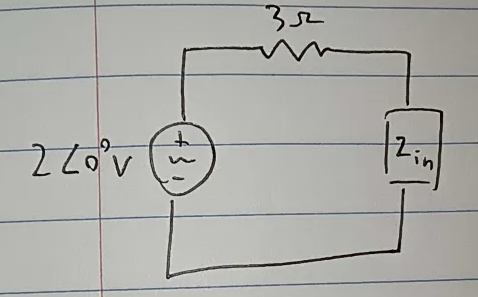
\includegraphics[width=0.4\textwidth]{13-41-1.png}
\end{center}
\[\implies \mathbf{Z_\text{eq}} = [3\,\Omega] + \mathbf{Z_\text{in}} = [3.00214\,\Omega]\]
\[\mathbf{I_1} = \frac{\mathbf{V_s}}{\mathbf{Z_\text{eq}}} = \frac{2\angle 0^\circ}{3.00214} = 0.666\angle 0^\circ\,\text{ A}\]
Using turns ratio, we can find $\mathbf{I_2}$:
\[\frac{1}{a} = \frac{\mathbf{I_2}}{\mathbf{I_1}}\]
\[\implies \mathbf{I_2} = \frac{\mathbf{I_1}}{a} = \frac{0.666\angle 0^\circ}{100} = 6.66\times10^{-3}\angle 0^\circ\,\text{ A}\]
Finally, we can directly calculate the average power dissipated by each resistor:
\[P_\text{avg} = \frac{1}{2}|\mathbf{I}|^2 R\]
\begin{itemize}
    \item $P_{\text{avg},\,3\Omega} = \frac{1}{2}[0.666\,\text{A}]^2[3\,\Omega] = \boxed{0.665\,\text{W}}$
    \item $P_{\text{avg},\,0.4\Omega} = \frac{1}{2}[6.66\times10^{-3}\,\text{A}]^2[0.4\,\Omega] = \boxed{8.87\times10^{-6}\,\text{W}}$
    \item $P_{\text{avg},\,21\Omega} = \frac{1}{2}[6.66\times10^{-3}\,\text{A}]^2[21\,\Omega] = \boxed{4.65\times10^{-4}\,\text{W}}$
\end{itemize}


\end{document}